\chapter{Managing e-Government}
Management of e-Government implementation involves the following:
\begin{multicols}{3}
	\begin{itemize}
		\item people
		\item process
		\item technology
		\item finance and
		\item partnerships
	\end{itemize}
\end{multicols}


\section*{Managing People}
e-Government has to be designed, developed, delivered and used by people --- people within government agencies, people outside the government in organizations that government would have to partner, citizens and business people. People management involves the following:

\begin{multicols}{2}
	\begin{itemize}
		\item Awareness building
		\item Education
		\item Training
		\item Coordination
		\item Team building
		\item Development of leadership qualities
	\end{itemize}
\end{multicols}


\section*{Managing Process}
\begin{itemize}
	\item \textbf{Service definition}: e-Government is about being service-centric.
	\item \textbf{BPR (Business Process Re-engineering)}
	\item \textbf{Legal process reform}
	\item \textbf{Delivery channel reform}
\end{itemize}


\section*{Managing Technology}
\begin{itemize}
	\item \textbf{Design and development of architectures}
	\item \textbf{Prescription of standards}
	\item \textbf{Security}
	\item \textbf{Procurement}
\end{itemize}

\section*{Financing e-Government Projects}
We need experts who can find innovative methods of financing e-government projects.

\section*{Managing Partnerships}
\begin{itemize}
	\item \textbf{Designing suitable partnership models}
	\item \textbf{Crafting the contracts}
	\item \textbf{Steering the partnerships}
\end{itemize}

 \section{Approaches to Management of e-Government Systems}
There are different ways in which management for e-government can be understood. Three possible approaches to e-government responsibilities (see Figure \ref{fig:e-government-approaches}):

%-----------------------------------
%		figure%
%-----------------------------------

\begin{figure}[tph]
	\centering
	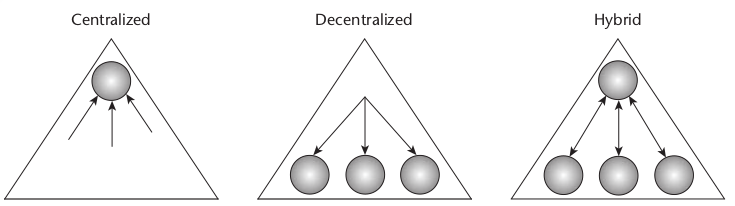
\includegraphics[width=0.9\textwidth]{e-government-approaches}
	\caption{Different approaches to e-government systems responsibilities}
	\label{fig:e-government-approaches}
\end{figure}
\begin{enumerate}
	\item \textbf{Centralized}: Decisions are taken at the most senior or central level.
	
	\item \textbf{Decentralized}: Decisions are taken at some level lower than the most senior; typically by individual work units within the organization or even by individual staff. The latter may also be referred to as end-user computing, where the individuals within the public sector who make use of outputs from e-government systems (the internal
	end users) are also those who operate and/or develop and/or manage those systems.
	
	\item \textbf{Hybrid}: Decisions are taken at both senior and lower levels, either separately or in an	integrated manner. This approach is called federal or federated in some governments.
\end{enumerate}

\subsection[Centralized Approach]{Centralized Approach to e-Government}
Some examples can be given of what a centralized approach to e-government would
mean. In terms of computing and data management architecture, a centralized computing architecture would be one which involves a large central computer with dumb terminals or network computers attached. That represents an internal view of architecture. An external view sees centralized data architecture in terms of portals: single central web locations through which all data is routed to users. 

Under a centralized approach, e-government systems are typically developed by a team from the central IT unit, or by external contractors under central IT unit control. The content and timing of individual projects can be drawn from any e-government strategy that has been developed. That strategy could also be used to guide procurement, where organization-wide
standards would be set for hardware, software and telecommunications equipment. Typically, a central group is responsible for setting standards, arranging contracts with suppliers, policing standards, and giving final approval on all IT purchase requests. Purchases of IT and IT budgets are routed through a central control point.

In a centralized approach, training is planned and prioritized organization-wide to fit in with e-government plans. Like technical support, it may be delivered by external providers or by specialist staff from the central IT unit. 

\subsubsection{Benefits of a Centralized Approach}

\paragraph*{Achievement of scale economies}
Centralized approaches allow most activities to be undertaken more cheaply per unit. Items purchased externally — computers, software packages, consumables, staff training, systems development, consulting, and so on — can be decided upon once and then bought in greater bulk.
Activities undertaken internally — from system development to implementation
and maintenance, and management of all these processes — cover a greater number of staff.

\paragraph*{Avoidance of duplication}
One main intention of centralized approaches is to have a single version of any particular e-government system for the whole organization, and to store any item of data once and only once. As a result, there is no wasted effort, no wasted storage
capacity, and no inconsistency of data. For example, only one accounting application needs to be developed for the whole agency. Similarly, if dealing with a set of external clients (such as businesses), each client’s name and details are captured once for use on a single, shared database. If these details change or if the required data structure changes, only one set of amendments needs to be made. The database represents the single authoritative source of digital information in the organization. This saves money, and can also improve data quality.


\paragraph*{Sharing resources}
A well-planned centralized system holds data used across the organization in one place, allowing all staff to access it. This makes it cheaper, faster and easier to undertake organization wide activities. Central planning and operation also allows compatible technology and skills to be introduced. Exchange of hardware, software and staff between
organizational systems and units therefore becomes much easier and less costly.



\subsubsection{Disadvantages of Centralized Approaches}

\paragraph*{Heavy time consumption}
Centralized decisions and actions can be
more time-consuming than for a decentralized approach because of: 
\begin{itemize}
	\item the additional time it takes for information to flow up the organization as an input to centralized decisions;
	\item the additional time it takes to collate information from a variety of different decentralized locations as an input to centralized decisions; and 
	\item the additional time it takes for implementation information to flow down the organization.
\end{itemize}


\paragraph*{Limited ability to meet user needs}
Centralized approaches necessarily mean that priority goes to those e-government systems which are seen as important by some select and centralized staff group. The priorities of the periphery – both individuals and individual work units inside government, as well as clients outside government may not be addressed.


\paragraph*{Inflexibility}
The greater the amount of central planning that has gone into an e-government system decision, and the longer that decision is therefore intended to provide guidance for the organization, the less flexibility it offers the organization to cope with differences between local units, or with internal or external changes.


\subsection[Decentralized Approach]{Decentralized Approach to e-Government}
Examples of a decentralized approach to managing e-government systems responsibilities
can be provided. In terms of computing and
data management architecture, a truly decentralized computing architecture would be one
that involves standalone computers or, possibly, a peer-to-peer network. Decentralized
approaches are commonly associated with the
spread of personal computers throughout an
organization. An external view would see
multiple websites and other routes through
which data could be accessed.

Under a fully decentralized approach,
e-government systems would be developed
within organizational work groups, focused
on their requirements, or even by individual
end users. Decentralized procurement means
that individuals or groups select and procure whichever technology best suits their
particular needs. Similarly, a decentralized
approach to training means that individuals
or small groups plan their own training
needs. It is likely that training takes place
on the job or through informal coaching of
one staff member by another.

\subsubsection{Benefits of Decentralized Approach}

\paragraph*{Greater fit between systems and local needs}

The closer the proximity of user and developer, the less the communication gap and
the more likely it is that the developed
system meets the users’ real needs.


\paragraph*{Faster system development}
The less the organizational distance between
system user and system developer, the faster
development of that system is likely to be.


\paragraph*{Perceived lower costs}
Decentralized approaches present lower costs than centralized approaches in certain areas. This is thanks to:
\begin{itemize}
	\item faster development, 
	\item less miscommunication, 
	\item greater fit to local needs through smaller design–reality gaps, 
	\item the greater emphasis on smaller computers, 
	\item the greater emphasis on buying software packages rather than developing software in-house, and so on.
\end{itemize}


\subsubsection{Disadvantages of Decentralized Approach}
\paragraph*{Barriers to sharing data}

Decentralized approaches can create e-government systems in different work units that are mutually incompatible.

\paragraph*{Barriers to sharing other resources, including human resources}
There may also be an inability to share
other resources if work units are allowed to
set up their own separate e-government systems. It may be hard to exchange hardware
and software. Perhaps more importantly,
each individual system requires a unique set
of skills for system development, implementation and operation. This makes it more
difficult for staff to move between different
e-government systems.


\paragraph*{Duplication of effort}
Decentralized approaches also tend to be very costly because units will often duplicate what others are doing.

Duplication covers analysis, design and implementation of e-government systems; gathering and administration of data; and system operation,
support and maintenance.

This imposes extra costs in gathering,
maintaining and updating data.

\paragraph*{Lack of learning and control}
In addition to the extra direct costs that
duplication imposes, there is an indirect
cost of lost learning opportunities and limited
cross-fertilization of ideas.



\subsection[Hybrid Approach]{Hybrid Approach to e-Government}
Both the centralized and
the decentralized approach to managing
e-government can provide benefits for public
organizations. Yet, at the same time, such
approaches can be hard or impossible to
implement, and can produce serious disadvantages for the organization.


What is the way out of this quandary?

One way forward is the adoption of a hybrid approach that attempts to reconcile the push of the centralized approach with the pull of the decentralized approach.



A hybrid approach to e-government can be feasible and
provide distinct benefits. A decentralized approach may be most economic for public
organizations, because it saves on overt input
costs. A centralized approach may be most efficient, because it avoids waste and duplication.
But a successful hybrid approach may be most
effective because it can simultaneously provide:

\begin{itemize}
	\item the control necessary to share key resources
	(including data), to avoid duplication, and
	to achieve economies of scale; and
	\item the freedom necessary to meet user
	needs, and to overcome blocks to IT
	usage and system development.
\end{itemize}



\subsubsection*{Examples}

\paragraph*{Computing and Data management architecture}
The most common hybrid computing architecture is the client/server model, in which computing power is divided between the central servers and the local client workstations. This architecture has now been adopted by vast numbers of public sector organizations worldwide.


A similar hybrid approach to portals
creates a single main portal which merely
links through to an existing set of sub-portals.


\paragraph*{Systems development}
A hybrid approach to systems development can involve a division of responsibilities; for example, defining certain types
of e-government system as suitable for
central development, and others as suitable
for decentralized/end-user development.

\paragraph*{Procurement}
Standards for procurement bring many
immediate and obvious benefits to public
agencies.

%--------------------------------end of section--------------------------
\section{e-Government Strategy}
An e-government strategy is a plan for e-government systems and their supporting
infrastructure which maximizes the ability of management to achieve organizational objectives. Increasing numbers of public agencies are developing an e-government
strategy.

\subsection*{Strategic Planning}
A set of core questions about e-government strategy for public agencies are:


\subsubsection*{Why?}
Why are increasing numbers of public agencies trying to develop an e-government strategy?

Following could be the explanations.
\begin{itemize}
	\item The fad/`me too’ factor of copying current trends or copying appearances in
	other organizations.
	\item The desire of some senior officials to wrest control of e-government from technical staff and/or individual departments.
	\item The desire for the kudos\footnote{An expression of approval and commendation} and resources associated with a major organizational
	initiative.
	\item The demand for such strategies from central government agencies.
\end{itemize}

In addition, the growth of e-government strategies in the public sector is
impelled by the potential benefits that a strategy can bring. 

Some of these are political, such as:
\begin{itemize}
	\item providing senior management control over organizational systems, 
	\item accessing central funds that are only	available on production of a strategy, and 
	\item avoiding public reprimands and penalties where strategies are demanded by higher level bodies.
\end{itemize}

An e-government strategy is also seen as
a key mechanism to produce centralized approach benefits


Finally, 
\begin{itemize}
	\item a successful strategy can develop
	senior management understanding that
	e-government systems are information
	systems not just IT.
	
	\item It permits a fundamental
	review of the organization’s use of information and technology, leading to a comprehensive understanding of information
	systems requirements. 
	
	\item It also provides a detailed plan of action on e-government for 	the organization.
\end{itemize}



\subsubsection*{What?}
Like any strategic plan, an e-government
strategy seeks to answer three questions,
illustrated in Figure \ref{fig:overview-of-strategic-planning}:
\begin{figure}[tph]
	\centering
	
\includegraphics[width=0.8\textwidth]{overview-of-strategic-planning}
	\caption{Overview of strategic planning}
	\label{fig:overview-of-strategic-planning}
\end{figure}

\begin{itemize}
	\item \textbf{Where are we now?} (i.\ e.\. how are systems working now, and what external factors affect them).
	
	\item \textbf{Where do we want to get to?} (i.\ e.\ in the future, how should the organization’s e-government systems be or work differently from at present).
	
	\item \textbf{How do we get there? }(i.\ e.\ what actions need to be undertaken to achieve the	outcome identified in answering the second question).
\end{itemize}


\subsubsection*{When?}
In simple terms, the answer is: ‘You undertake e-government strategy when the time
is right’.

In other cases, we undertake e-government strategy when:
\begin{itemize}
	 \item e-government systems being created without consideration for overall organizational objectives;
	\item outdated systems still in use due to inability to plan alternatives;
	\item data that cannot be shared between different e-government systems because
	there are no organization-wide standards;
	\item IT being seen as the end rather than the means; in other words, when
	e-government is seen as an end in itself;
	\item no clear locus of responsibility for dealing with these problems;
	\item comparative organizations have a strategy.
\end{itemize}

\subsection{Steps of e-Government Strategic Planning}
eGovernment strategic planning is typically conceived as a series of steps that are
undertaken systematically over a period of a few weeks or a few months. These steps are
summarized in Figure \ref{fig:steps-e-gov-planning}. Once completed, they produce a framework for organizational action that can endure for a number of years.

\begin{steps}
	\item Create e-government planning structures/roles
	\item 
	\begin{enumerate}[label=\alph*.]
		\item Audit information	systems
		\item Get guidance from	organizational strategy
	\end{enumerate}
	\item Set e-government objectives and principles
	\item 
	\begin{enumerate}[label=\alph*.]
		\item Determine e-government systems architecture
		\item Determine e-government organizational architecture
	\end{enumerate}
	
	\item Disseminate and plan e-government actions
	\item Manage, evolve and review e-government strategy
	
\end{steps}

\begin{figure}[hpt]
	\centering
	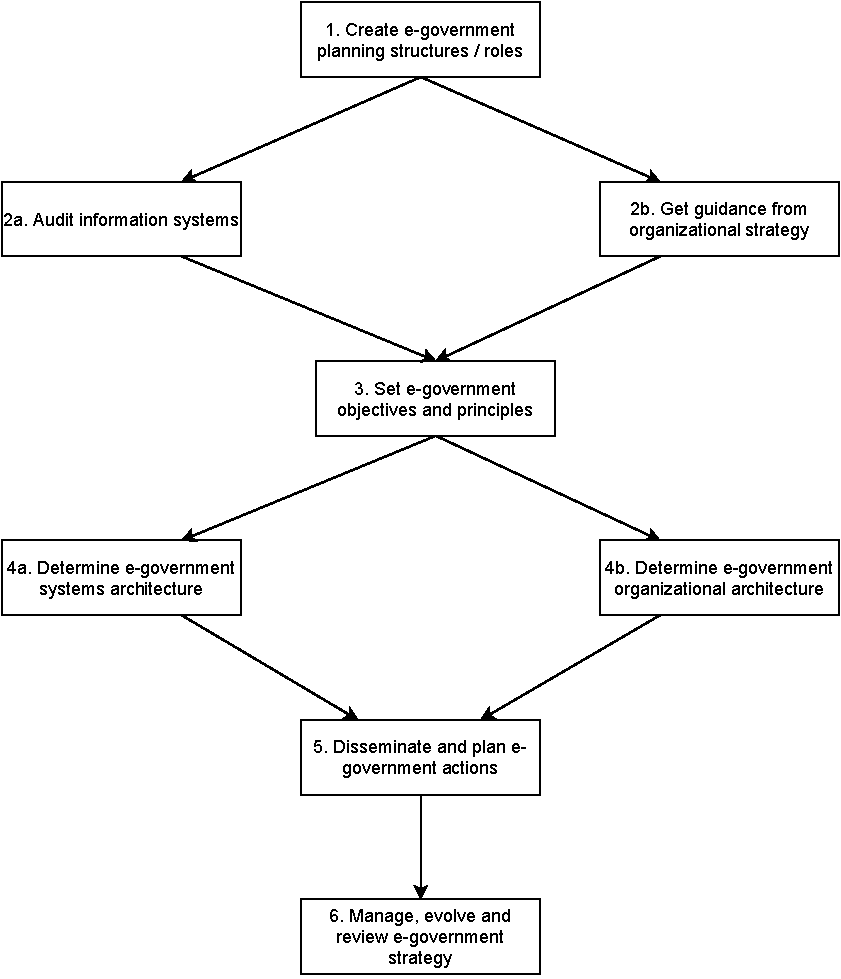
\includegraphics[width=0.9\textwidth]{steps-e-gov-planning}
	\caption{The steps of e-government strategic planning}
	\label{fig:steps-e-gov-planning}
\end{figure}

\subsubsection{Strategy Foundation: Create eGovernment Planning Structures/Roles}
\begin{itemize}
	\item In order to control the process of strategic planning, a special body is usually set up,	called something like `eGovernment Steering Group’. 
	\item It will typically consist of senior staff or other powerful stakeholders
	from various parts of the organization, together with some technical advisors.
	\item this committee is likely to be chaired by a Chief Information Officer
	(CIO).
\end{itemize}

This body normally reports to the very
top levels of the organization because of the
strategic nature of its work, which includes:

\begin{itemize}
	\item setting the scope of, and commissioning the e-government strategy; 
	\item taking necessary strategic decisions relating to e-government systems (such as those presented during strategic	planning); 
	\item communicating the e-government strategy to the rest of the organization; \item ensuring the necessary resources are in place to achieve strategic objectives, and allocating those resources; and 
	\item monitoring and controlling the overall development and operation of
	e-government within the organization, and
	checking this against stated objectives.
\end{itemize}

\subsubsection{Strategic Analysis: Audit Information Systems}
An e-government-specific answer to the
question ‘Where are we now?’ requires a
comprehensive understanding of the current
state of e-government and other information
systems.

It includes all types of information system, manual or computerized: hence the title ‘audit information systems’ rather than ‘audit e-government’.


Information systems (IS) audit is often
conceived in a very narrow sense, just as
an inventory of IT within the public
agency: all computer applications with
their hardware, software, networks, physical location, licensing and ownership; and
often just security-related. However such an approach is far too narrow to form an effective analytical base for strategy. It must be expanded in several ways, as below:

\paragraph*{Systems perspective}
Audit must recognize the full information system, describing not just the technology resources, but also: 
\begin{itemize}
	\item the information that information systems deliver, 
	\item the information processes undertaken, and 
	\item the human resources involved,
	\item covering information skills (e.\ g.\ data gathering and presentation), IT skills (e.\ g.\	hands-on computing), and system development skills (e.\ g.\ systems analysis and design).
\end{itemize}


\paragraph*{Issues perspective}
The audit should be more than just a list of
resources, but should help identify key
issues that will inform and affect subsequent decision-making on e-government.
These might include a sense of important
problems or complaints facing the current
information systems, or an assessment of
emerging trends.

\paragraph*{Contextual perspective}
This includes the outer two layers of the
‘onion-ring’ (see Section \ref{sec:e-gov-as-information-system}) within the
audit.

\begin{itemize}
	\item It will look at management systems and structures within the public agency.
	\item It will look at IT trends and standards within the local environment. 
	\item It will review financial and other constraints specific to e-government systems change. 
	\item Perhaps most important, it will incorporate an understanding of relevant policies, guidelines and initiatives that impact on	e-government. 
\end{itemize}


\subsubsection{Strategic Analysis: Get Guidance From Organizational Strategy}
An e-government strategy should therefore be firmly rooted in one particular element from the organizational context: the wider organizational or business strategy for the whole agency.

Business strategy first asks, 
\begin{itemize}
	\item `Where are we now?’ An answer	would include details of the organization’s	current structure and functions; key client	groups; existing problems that need to be addressed; and important current and forthcoming factors – particularly policies and political priorities – within the internal and
	external environment.
	
	\item It next asks, `Where do we want to get to?’ An answer would include details of the organization’s objectives, and some vision
	of the future organization that will enable it to overcome current and forthcoming problems, and to achieve its objectives.
	
	\item Finally, it asks, `How do we get there?’ This would be achieved through a statement of management strategy about major changes to
	organizational structure and functions in order to reach its future vision.
\end{itemize}

\subsubsection{Strategy Framework: Set eGovernment Objectives and Principles}
The eGovernment Steering Group may use the data gathered so far to produce a broad statement of the role and objectives of information and of e-government within
the organization. This statement may be specific (tying e-government to particular organizational objectives) and/or it may be generic (a general statement of information
and IT principles). 


These objectives and principles can also be used to develop the criteria against which e-government proposals may be evaluated and/or prioritized.


\subsubsection{Strategy Definition: Determine eGovernment Systems Architecture}
eGovernment strategy can be seen as needing to lay out the ITPOSMO dimensions for the future (see Section \ref{sec:e-gov-as-information-system}) The information,
technology and process dimensions are
together seen as an \textit{e-government systems architecture}: a plan of the e-government systems that the organization will require in
future. This architecture forms a major element of ‘Where do we want to get to?’ for
e-government.


The e-government systems architecture
can be described in terms of the individual
e-government applications with details of
data capture, input, processing, storage and
output plus links to decision and action
processes (CIPSODA: see Section \ref{sec:e-gov-as-information-system}) 

It will also consist of a number of different models, including:

\paragraph*{Data model}
\begin{itemize}
	\item A data model showing the structure of unified, organization-wide data to
	which the e-government systems will	have access; 
	\item often illustrated using an entity-relationship diagram.
\end{itemize}

\paragraph*{Process model}
\begin{itemize}
	\item A process model showing the key activities of the organization that the e-government systems will either support or undertake; 
	\item often illustrated using a process	diagram.
\end{itemize}


\paragraph*{Data/Process model}
\begin{itemize}
	\item A data/process model showing the organization-wide connection between
	business processes and data entities, and the organization-wide movement of data
	that e-government systems will enable;
	
	\item often illustrated using a data flow diagram.
\end{itemize}


The e-government systems architecture will
also consist of organization-wide models
for:

\begin{itemize}
	\item \textbf{IT}, showing how computers will be sized
	and connected within the organization,
	and an outline of the software to be used;
	\item \textbf{data management}, showing how data
	capture, input, processing, storage and
	output functions will be divided across
	the IT architecture.
\end{itemize}

A summary of all the elements within the
e-government systems architecture is shown
in Figure \ref{fig:architecture-elements-e-gov}.


\begin{figure}[ht!]
	\centering
	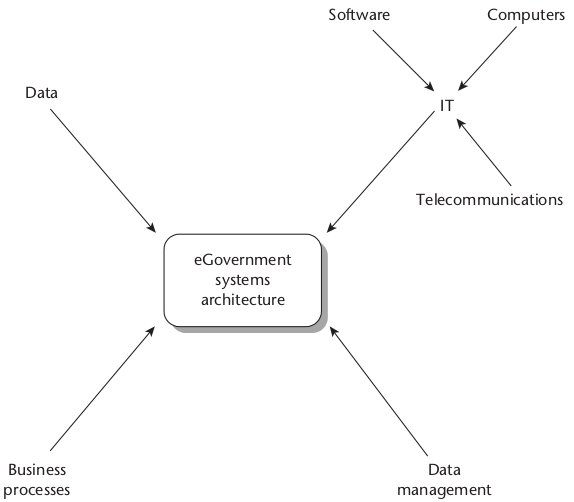
\includegraphics[width=0.8\textwidth]{architecture-elements-e-gov}
	\caption{Elements of e-government systems architecture}
	\label{fig:architecture-elements-e-gov}
\end{figure}


\subsubsection{Strategy Definition: Determine eGovernment Organizational Architecture}
General strategic decisions may include:

\begin{itemize}
	\item stating the approach to management of	organizational change, including a determination of the needs for cultural
	change;
	\item clearly allocating responsibilities for e-government systems development and
		management;
	\item identifying major competency gaps and	approaches to closing them through human resource strategies;
	\item deciding how back-office procedures may be restructured to support e-government;
	\item locating the e-government/IT function	within the wider organizational structure;
	\item demarcating which services (e.\ g.\ systems development, training and systems operation) are to be sourced in-house and outsourced;
	\item identifying procedures to be used when tendering for and selecting e-government systems products and services;
	\item specifying standard systems development methodologies and tools to be used; and
	\item identifying financial approaches to be adopted, such as public–private partnerships.
\end{itemize}


\subsubsection{Strategy Implementation 1: Disseminate and Plan eGovernment Actions}

The defined strategy can now be circulated as an ‘eGovernment Strategy Statement’ and,
if appropriate to the organizational culture, discussed and refined. 

Once agreed, the strategy is typically planned in more detail in a matrix format.

The columns of the matrix can be a set of e-government project plans, created for
improving existing systems and developing new systems. This might include:

\begin{itemize}
	\item a statement of project objectives; 
	\item an estimation of benefits, risks and constraints; and
	\item an estimation of resource requirements covering finance, human resources (i.\ e\. jobs and skills), technology, and timescales.
\end{itemize}

The rows of the matrix will be organization wide resource plans: 
\begin{itemize}
	\item for personnel training
	and development, 
	\item for finance, 
	\item for technology, etc.
\end{itemize}

\subsubsection{Strategy Implementation 2: Manage, Evolve and Review	eGovernment Strategy}
Strategic planning is not intended to be a
one-time activity but a continuous cycle
that needs to be completely revised at the
end of the strategic framework period, or
earlier if circumstances change or objectives
are not attained.

One task of the eGovernment Steering
Group is to monitor implementation of the strategic plan. Monitoring gathers
information on:

\begin{itemize}
	\item performance against objectives set for both e-government overall and individual
	e-government projects;
	\item benefits accruing to the organization	from e-government systems;
	\item problems related to developing or	operating e-government systems, with
	diagnoses and proposed remedies;
	\item other	impacts	associated with	e-government systems;
	\item changes to significant internal and external factors that affect the performance of the organization; and
	\item resources used and projected for use
\end{itemize}



On the basis of the information gathered, the eGovernment Steering Group may decide to modify the strategy.
%--------------------------------section end-------------------------




\section{Managing Public Data}
e-government systems are information systems. The data in e-government systems is therefore fundamental to the functioning of the public sector. It is too easy to assume that all is well with this data. Yet most e-government systems have data quality problems; sometimes so bad that they undermine the whole edifice of government functioning.

We can define data quality in terms of five `\textbf{CARTA}' indicators:

\begin{enumerate}
	\item \textit{\textbf{C}ompleteness}
	
	The degree to which all the data required by users is present in the e-government system.
	
	\item \textit{\textbf{A}ccuracy}
	
	The level of errors/incorrect data within the overall system data.
	
	\item \textit{\textbf{R}elevance}
	
	The degree to which data is necessary in order to complete particular	user decisions and actions.
	
	\item \textit{\textbf{T}imeliness} 
	
	The degree to which data can be delivered by the e-government system within a required time-frame.
	
	\item \textit{\textbf{A}ppropriateness of presentation} 
	
	The degree to which data produced by the	e-government system is accessible and intelligible to the recipient.
\end{enumerate}

\textit{The more CARTA the data, the higher its quality; the less CARTA the data, the lower its quality.}



It is estimated that around higher percentage of system data errors arise during the human elements of the process. Historically, this has occurred mainly during capture and input, because these were traditionally human-intensive tasks with errors arising from misreading, mistyping, and lost or omitted inputs. It has also
occurred after output, also because of misreading or misunderstanding.

But data errors can occur at any stage in the information cycle, for example, during processing, storage, output or transmission between those stages, as illustrated in Figure \ref{fig:poterntial-data-error-in-e-gov-cycle}.


\begin{figure}[th!]
	\centering
	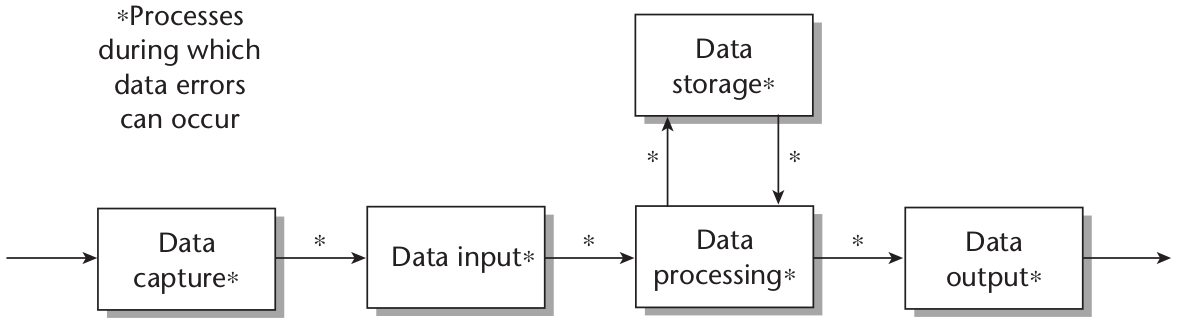
\includegraphics[width=0.8\textwidth]{potential-data-error-in-e-gov-cycle}
	\caption{Potential data error points in the e-government system cycle}
	\label{fig:poterntial-data-error-in-e-gov-cycle}
\end{figure}

In all cases, the data output will not be accurate or reliable. eGovernment systems with poor data will be prone to collapse as the poor data foundation undermines decision-making and action, as summarized in Figure \ref{fig:impact-of-inaccurate-data}.


This is often described as \textit{garbage in, garbage out (GIGO)}: what you get out from your e-government systems can only ever be as good as what you put in, and
if you put in garbage, you get out garbage. 

This is an issue for all organizations, but it is particularly an issue for the public sector and e-government:
\begin{itemize}
	\item The public sector is especially information intensive, and therefore relies heavily on data in order to undertake its	functions.
	\item The public sector often has responsibility for decisions that are critical to an individual's, a region’s or a nation’s welfare. 
	\item The public sector has legal obligations relating to data quality and accessibility, for example in relation to freedom of	information. 
	\item It therefore faces a significant threat of litigation if data quality is poor.
\end{itemize}

\begin{figure}[ht!]
	\centering
	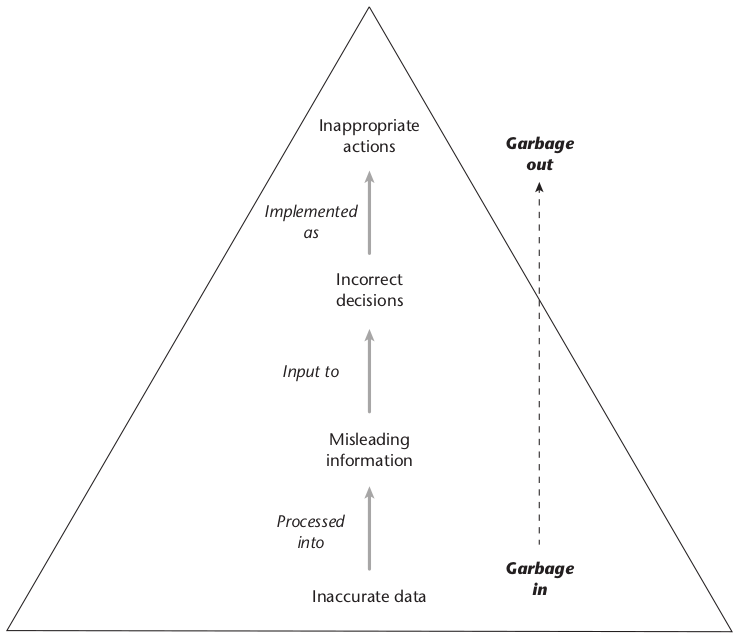
\includegraphics[width=0.7\textwidth]{graphics/impact-of-inaccurate-data}
	\caption{Impact of inaccurate data}
	\label{fig:impact-of-inaccurate-data}
\end{figure}

The public sector may also face additional constraints — on skills, on technology, related to the large size of its data sets — that increase the risks of data quality problem

\subsection{Causes of Public Data Problems}
We can divide causes into two main camps: 
\begin{enumerate}
	\item \textbf{hard}: technical causes of data quality problems and 
	\item \textbf{soft}: human causes. 
\end{enumerate}


\subsubsection[Technical Causes]{Hard Side: Technical Causes}
Looking first at the hard side, one can see that public managers love to blame data glitches on `computer errors', and that some technical problems do arise
which affect the data held by IT:


\paragraph*{Environmental hazards}
\begin{itemize}
	\item High temperatures and high humidity can cause hardware components to break down, thus corrupting data. 
	\item Static electricity can damage both electromagnetic components and corrupt data.
	\item Dust and smoke can short out components and make moving parts stick, especially damaging disk drives and the data on them. 
	\item Fire,	flood and lightning have a fairly obvious and catastrophic effect on IT-based systems.
\end{itemize}

\paragraph*{Electrical Problem}
\begin{itemize}
	\item Power spikes or surges (increases in voltage), and brownouts (decreases in voltage) can corrupt disk	held data and damage internal components. 
	\item Power cuts cause an ability to work, and a loss of all data in memory.
\end{itemize}


\paragraph*{Equipment breakdown} This can prevent data being exchanged or accessed.


\paragraph*{Software errors}
\begin{itemize}
	\item The presence of bugs (programming errors) in the software of an e-government system can have any number of effects. 
	\item These include overt or, worse, undetected corruption of data.
\end{itemize}


\noindent But to what extent can these truly be classified as `computer errors’ or technical problems? 

\subsubsection[Human Causes]{Soft: Human Causes}
The presence of bugs should be seen mainly as a problem of human, rather than technical, origin relating to the management of systems development. Even the actions of environmental or power hazards can often be traced to human inputs in the design, construction or operation of IT-based systems. This must put a question mark over the value of some hard approaches to public data quality.

We can reinforce this point by looking at another way in which technology could be blamed for inducing a further vulnerability and danger to data accuracy: the threat of computer crime.

Computer crime is a major problem for the public sector: 

\begin{itemize}
	\item internally, public employees are a significant source of such crime; 
	\item externally, threats seem to be growing and cyber-security has risen sharply up the agenda in many countries as a result of the terror attacks of the early $ 21^{st} $ century.
\end{itemize}


As well as entry of inaccurate data onto computer systems for personal gain, computer crime also includes:

\paragraph*{Alteration of existing data}
 For example, a worker increasing the rate of pay recorded for them in the payroll system, or the defacing.
 
 \paragraph*{Unauthorized access to existing data}
Hackers getting access to critical public data.

 \paragraph*{Deliberate destruction of data}
 For example, removing part of the organization's financial records just for the hell of it or introducing a computer virus.



\noindent Computer crime also covers physical theft of computer hardware or software (software piracy). Some public agencies even include personal use of organizational IT, such as typing and printing a personal letter or buying goods on the web from your office PC.


\subsubsection[Hard Solutions]{Hard Solutions to Public Data Quality Problems}
Hard, technical response to problems of data accuracy, including computer crime requires the imposition of various controls. These can be divided into two groups: 
\begin{enumerate}
	\item \textbf{general controls}, which affect all e-government systems; and 
	\item \textbf{application controls}, which relate to one particular e-government system.
	
\end{enumerate}


\paragraph*{General controls}

\begin{itemize}
	\item \textbf{Access controls}:
	\begin{itemize}
		\item Used to control user access to physical or digital components	of an e-government system. 
		\item Examples include security guards and passwords.
	\end{itemize}

\item \textbf{Communication controls}:
\begin{itemize}
	\item Used to control user access over computer networks.
	\item Examples include encryption and firewalls.
\end{itemize}
\item \textbf{Other technology controls}:
\begin{itemize}
	\item Such as controls to address virus, fire or power issues.
\end{itemize}
\end{itemize}


\paragraph*{Application controls}
To prevent many kinds of problems, many public agencies use application controls. The most important of these are \textbf{input controls}; that is, controls on the process of data entry that can be built into the e-government system. In many cases, if the control is violated, a customized message will appear providing guidance on the problem, and the new record will not be accepted until the error is corrected. 

Typically, the controls operate on each field within a database record and are stored as rules associated with that field.


\subsubsection[Soft Solutions]{Soft Solutions to Public Data Quality Problems}
We could identify a different role for each one of the CIPSODA (see Section \ref{sec:e-gov-as-information-system}) elements of an information system. However, that model can be simplified somewhat to produce the summary shown in Figure \ref{fig:data-roles}. This removes the roles of storage and output (because technology normally fulfils those roles) and merges the roles of decision maker and actor into the term `user'.


\begin{figure}[bh!]
	\centering
	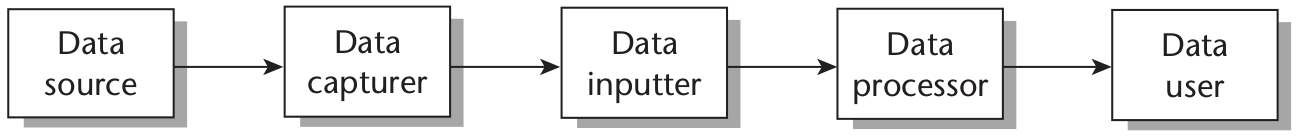
\includegraphics[width=0.8\textwidth]{data-roles}
	\caption{Different data roles played by people in public data systems}
	\label{fig:data-roles}
\end{figure}


The people occupying each one of these roles will have a different perspective on data, and we can develop a simple model of this, shown in Figure \ref{fig:soft-perspective-on-data-quality}. The model sees perceptions about how data is or is not used as shaping the motivations of each stakeholder which, in turn will shape their actions which, in turn will have an impact on data quality.


\begin{figure}[ht!]
	\centering
	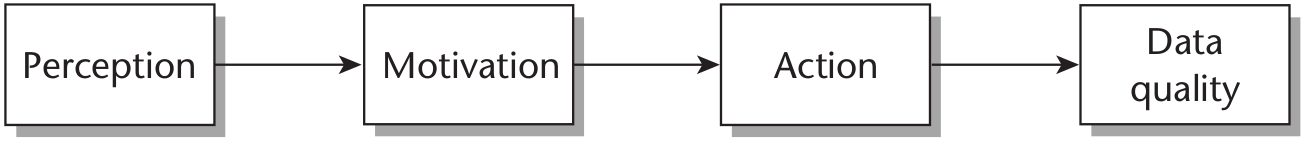
\includegraphics[width=0.8\textwidth]{graphics/soft-perspective-on-data-quality}
	\caption{A soft perspective on data quality}
	\label{fig:soft-perspective-on-data-quality}
\end{figure}

The soft perspective therefore argues that one of the keys to data quality, or lack of it, lies in the motivations of those involved. Where they are motivated to do so, those
involved will help data quality to be high. Where they are motivated to do otherwise, data quality is likely to suffer.


Some examples of perceptions — and their related motivations — will illustrate:

\paragraph*{Perception of data irrelevance}

\begin{itemize}
	\item Sources in public data systems, such as those asked to take part in a census or other survey, are often asked to provide data that is for the use of someone other than themselves. 
	\item Similarly, those capturing, entering and processing data are often treated as clerical automata, merely transmitting data to be used by some senior official. In such
	situations, the humans involved see the	data as largely irrelevant to their own work and their own lives, because they never use it. 
	\item As a result, they have limited motivation to worry about data quality, and their actions — for example, lack of care in response, or lack of concern about data entry errors — may undermine data quality.
\end{itemize}


\paragraph*{Perceptions of non-use}
This is related to the perception of data irrelevance. 

\begin{itemize}
	\item In some e-government systems, those involved know (or believe) that the data they are giving or collecting or inputting or processing is never actually going to be
	used. 
	\item This will have a knock-on effect on data quality.
	\item Within the politicized context of the public sector, for example, data entry staff may know that the data they type in is not	used; perhaps because senior officials make decisions using informal, political data rather than rational data from the computerized e-government system. 
	\item In that case, perfectly logically, the data entry staff will not be motivated to care about ensuring accuracy of the data they type in. 
	\item Alternatively, take the case of residents asked to provide input to the planning of a community policing strategy.
	\item Having once taken the trouble to provide data, they might feel that their efforts have produced no discernible result if no sensible strategy emerges. 
	\item Feeling their data was not going to be used they might, in the future, be motivated to refuse to provide further data to the police service.
\end{itemize}



\paragraph*{Perceptions of data-related punishment}

\begin{itemize}
	\item Citizens and businesses perceive that providing accurate financial data will lead to a punishment: their having to pay tax. 
	\item They are therefore motivated to withhold data (by	not providing a tax return, or not providing a full tax return); or to distort data (e.\ g.\ to	underestimate their income/profit or overestimate their expenditure/losses). 
	\item Any situation in which information is felt to have a political value may also lead to it being withheld on grounds of the old adage `information is power'.
\end{itemize}


\paragraph*{Perceptions of other data-related rewards}
\begin{itemize}
	\item Where performance-related pay has been instituted in the public sector, staff will rightly perceive that the provision of certain performance data (i.\ e.\ apparent performance above target) to their managers will lead to some personal reward (i.\ e.\ a pay bonus). 
	
	\item In this situation they will be motivated to hide negative performance data and to inflate or make up positive performance data, thoroughly undermining the performance management system. 
	
	\item Conversely, political leaders may be motivated to paint a falsely negative picture of difficulties in their district if they believe this will trigger a flow of assistance and development resources from federal or international funds.
\end{itemize}


\noindent These reward and punishment perceptions particularly affect the public sector and its clients (to whom it will often be providing money, services or other resource rewards), and compliers (whom it will often be `punishing' via a gamut from tax bills through fines or license revocation up to imprisonment). In all these cases, the citizen’s self-interest dictates that they will not be motivated to not present or handle data accurately.


All this assumes that those involved do have some perceptions, but there may be situations in which there is a lack of perception; for example, where sources do not know why data is being sought from them. They will try to work this out from situational clues, but they may guess wrong and accordingly skew the data they provide wrongly. Equally, there can be cases of lack of knowledge; for example, where sources feel motivated to provide data even though they do not have that data.


\subsubsection{Improving Public Data Quality}
what would the soft approach advocate as a way to address data quality problems in e-government systems? The key will be the perceptions and motivations of all those
involved in the chain. In particular, the public agency needs to find ways to align perceptions and personal motivations with formal organizational objectives.

What mechanisms exist for doing this? Some suggestions follow, summarized in Figure \ref{fig:soft-approach-data-quality}.
\paragraph*{Ensure there is a user}
\begin{itemize}
	\item Perception of data non-use is a major demotivator. 
	\item Matters can be improved if the e-government system is redesigned to ensure that the data being gathered is actually used for decisions and actions. 
	\item This may involve changing the content of data gathered to match the true information needs of users.
\end{itemize}

\paragraph*{Merge stakeholder roles}
\begin{itemize}
	\item The greater the number of stakeholders in the chain, the greater the chance of motivational problems. 
	\item Merging roles will reduce this danger. 
	\item Those who capture the data can also be those who input the data. 
	\item For example, where a survey was being	undertaken, role merger could mean the use of handheld devices that can accept data input in the field.
	\item Going further, data sources can themselves capture and input data.
	\item Where the consumers of public services themselves become producers of their own data, the use of web-based electronic	forms enables this.
\end{itemize}

\paragraph*{Make early stakeholders into data users}

\begin{itemize}
	\item Sources, capturers and inputters typically do not use the data that depends on them. 
	\item If they are turned into users, they have a much greater motivation to ensure the quality of system data.
\end{itemize}


\paragraph*{Other feedback to early stakeholders}
\begin{itemize}
	\item Even if early stakeholders do not become data	users, other types of feedback can motivate them. 
	\item This can be as little as a simple word of thanks from the user, or an explanation of why and how the data	is being used.
\end{itemize}

\paragraph*{Other reward and punishment techniques}
\begin{itemize}
	\item Giving money to data sources and higher pay to data capturers, inputters and	processors is one motivational technique, but money is not the only motivator.
	\item Punishment too can play a role, such as realistic threats of fines or imprisonment for those failing to fill or filling inaccurate tax returns, or threat of removal/reduction of budget by an audit or for failure to produce accurate audit figures.
\end{itemize}

\paragraph*{Find alternative sources}
\begin{itemize}
	\item Identify alternative sources for the same or similar data, who/which have less self-interest in the use of the data.
	\item For example, get administrative staff to return data on service activities of professionals (e.\ g.\ number of clients met) rather than the professionals themselves.
\end{itemize}


\begin{figure}[th!]
	\centering
	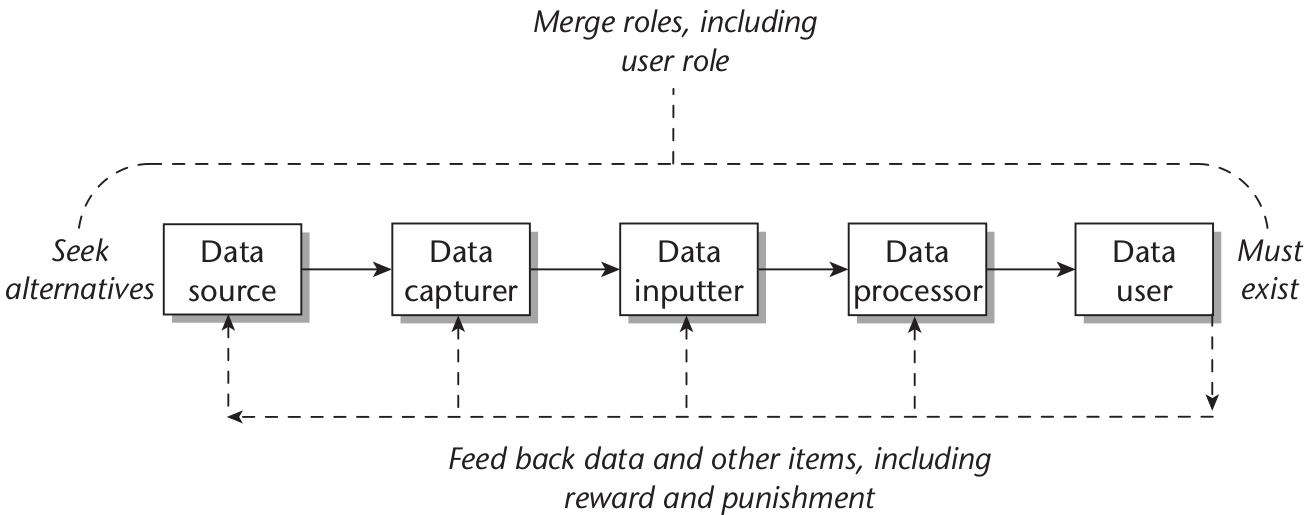
\includegraphics[width=0.9\textwidth]{graphics/soft-approach-data-quality}
	\caption{Soft approaches to improving data quality}
	\label{fig:soft-approach-data-quality}
\end{figure}



 %--------------------------------section end-------------------------
 
 \section{Managing Issues for e-Government}
 
\subsection{Core Issues}
Following are core issues that managers in the public sector have always faced:
\begin{itemize}
	\item position (the location of the IT function	within public sector organizations);
	\item people (recruitment and retention of staff involved with e-government);
	\item pelf (dealing with the financial aspects of e-government);
	\item projects (the ways in which e-government projects are managed);
	\item politics (the role of organizational power and politics in e-government).
\end{itemize}

\subsubsection{Position}
Where in the organization is the IT function to be located? There are various different possibilities.
\begin{itemize}
	\item Decentralized location,
	\item Centralized location,
	\item Hybrid approaches to IT location.
\end{itemize}

\paragraph*{Decentralized location}
At the extreme, responsibilities for e-government may be so decentralized that no organizational IT structures, staff or budgets exist: everything is left up to individual staff. 
\begin{itemize}
	\item One stage up from this is the situation in which one member of staff in each section is identified as the computer ‘whizz-kid’. 
	\item While continuing to perform their usual managerial or clerical role, they	informally take on an IT1 support role. 
	\item One stage further up, some or all of the organization’s departments have their own IT staff and/or IT unit and a specific departmental IT budget. 
	\item These resources are focused on serving the needs of the individual departments.
\end{itemize}


\paragraph*{Centralized Location}
At the other extreme is the centralized IT unit. 

\begin{itemize}
	\item Such units are normally funded from a	central budget. 
	\item They are naturally larger than their decentralized counterparts. 
	\item They may therefore be divided internally into a number of sub-units covering specialisms such as computer and network operations, systems development, data management, and strategic planning.
\end{itemize}

The location of the IT unit within the
overall structure of the organization reflects
attitudes to e-government in the organization, and also partly determines what the
unit can and cannot achieve within the
organization.


\paragraph*{Hybrid approaches to IT location}
Looking within the public agency, a hybrid location can mean either a separation or
integration of central and local responsibilities. For example, there could be a hybrid
management structure for the IT unit, with a management group that involves internal
users and senior officials as well as IT staff.

Alternatively, a hybrid structure for the IT unit could mean that it reflects the wider
structure of the public agency. Thus, for example, a unit supporting a local government could have a team covering housing, another team covering public works, another covering environment, and so on.


\subsubsection{People}
People are more important than technology. eGovernment managers must therefore spend much of their time dealing with people related issues.

The planning, development and operation of any new e-government system is likely to require new competencies, thus creating a gap between the competencies staff currently hold and those they need.

Competencies can be understood in relation to three domains:
\begin{enumerate}
	\item \textbf{Skills}: Organizations may find a skills gap in anything 
	\begin{itemize}
		\item from spotting opportunities for new e-government systems, 
		\item to analyzing current use of information, 
		\item to process redesign, 
		\item to software programming, 
		\item to system installation and use.
	\end{itemize}

	\item \textbf{Knowledge}: Organizations may therefore find a knowledge gap where staff do not know:
	
\begin{itemize}
	\item about systems development methods, or 
	\item about the nature and role of information and information systems, or 
	\item about organizational systems and processes, or 
	\item about	the basics of IT, or 
	\item about the design options that could be applied to the new e-government system, or 
	\item about why the new system should be operated in a particular way.
\end{itemize} 

\item \textbf{Attitudes}:
\begin{itemize}
	\item Where different stakeholders have different attitudes to the new e-government system, 
	\item one could talk of	an `attitude gap'. 
	\item In many ways this	reflects the different values and objectives of different stakeholders.
\end{itemize}
\end{enumerate}


Public managers face two main options in filling these competency gaps that new e-government systems create. They can:
\begin{enumerate}
	\item Train existing staff,
	\item Recruit new staff.
\end{enumerate} 


\subsubsection{Pelf}
Money matters loom large in e-government projects. For example, e-government has to work within the confines of public sector budgeting procedures. Related to this, e-government also has to work within the confines of available finance.

 \subsubsection{Projects}
The overriding management issue for e-government projects should be the challenge of failure. 
\begin{itemize}
	\item Most e-government initiatives fail due to poor implementation and management.
	\item Gaps between design and reality help to explain why e-government systems succeed or fail.
\end{itemize}


\subsubsection{Politics}
e-government is far more about people and politics than it is about technology and rationality:

Sometimes, IT projects fail because of economic reasons; rarely, if ever, because of technological factors. Most usually, the failures are political in nature.

Why should there be so much politicking around e-government? In short, because two pre-conditions of politicking\footnote{the action or practice of engaging in political activity.} are met.

\begin{enumerate}
	\item First, there are interdependent groups that have different objectives and values. 
	\item Second, there are important but scarce resources involved.
\end{enumerate}

So e-government brings together in large amounts both critical tangible resources — people, money and equipment — and critical intangible resources — information, power and kudos. They therefore form a key locus\footnote{a center of activity, attention, or concentration} for organizational politics.

%--------------------------------section end-------------------------


\section{Emerging Management Issues for e-Government}

Followinga are the management issues that have come to prominence more in recent years. 
\begin{enumerate}
	\item \textbf{performance} (the measurement of e-government-related performance);
	\item \textbf{policies} (the organizational policies that e-government managers have to develop	and promote); these are divided into:
	\begin{itemize}
		\item \textbf{policies on public data}, and 
		\item \textbf{policies on	other issues}.
	\end{itemize}
	 
\end{enumerate}

 \subsection{Performance}
 \begin{itemize}
 	\item Performance management is a component of public sector reform. 
 	\item It is a technique originating in the private sector that is now being promoted in the public sector. 
 	\item As with most such techniques, issues arise because some of the assumptions underlying performance management do not apply, or apply differently, in the public sector.
 \end{itemize}

\begin{figure}[ht!]
	\centering
	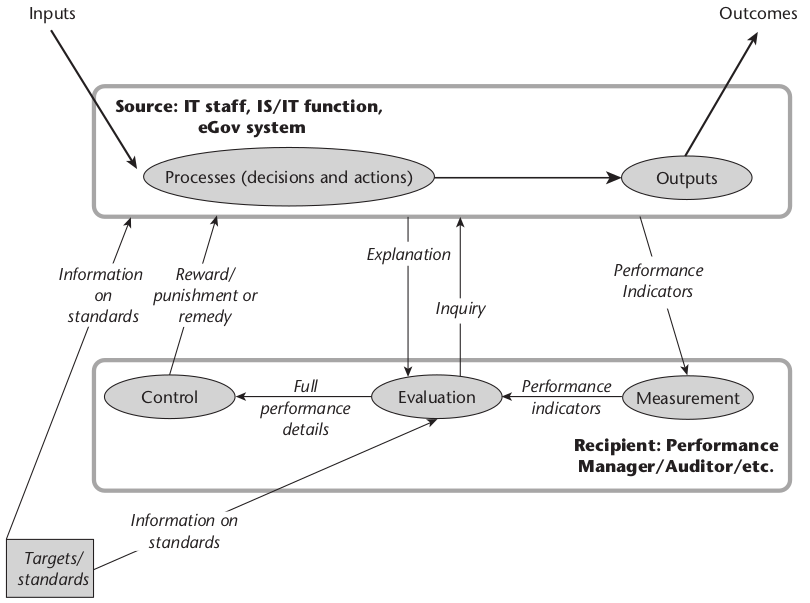
\includegraphics[width=0.8\textwidth]{perfromance-management}
	\caption{Performance management in e-government}
	\label{fig:perfromance-management}
\end{figure}

\subsubsection{Staff Performance}
Performance management in the public sector follows a standard pattern of target
setting, measurement, evaluation and control, as shown in Figure \ref{fig:perfromance-management}.


\begin{itemize}
	\item In reference to IT staff management, this would involve working first on a clear job specification and then tying the major items of content (ideally those that are output related) down to measurable performance indicators and targets. 
	\item Actual measures of performance would typically be discussed as part of regular staff-manager meetings with reasons for under and over-achievement discussed. 
	\item Rewards would be instituted for achievement/over achievement and remedial measures for
	under-achievement.
\end{itemize}

\subsection{Policies}
\subsubsection{Policies on Public Data}
 Public agencies operate in a sea of government laws, orders, policies and regulations. These external drivers pressurize agency e-government managers to develop and implement their own internal policies on
 a wide variety of issues.

Data policies must grapple with a four way data conflict faced by public agencies, summarized in Figure \ref{fig:data-conflicts}.

\begin{figure}[th]
	\centering
	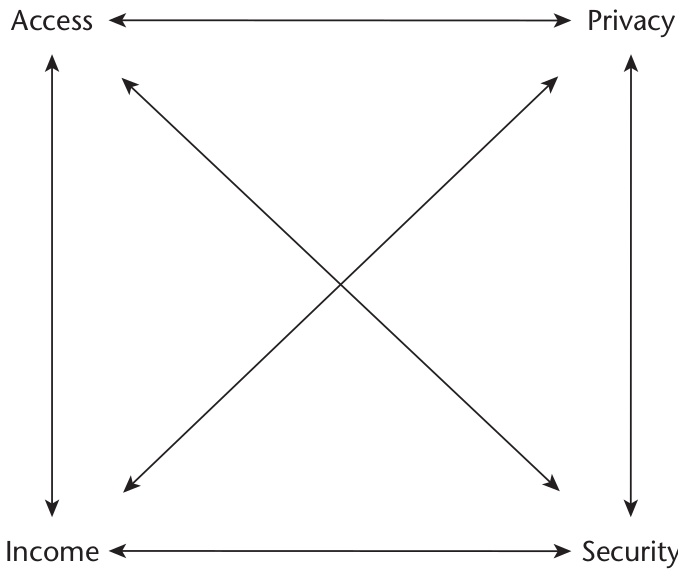
\includegraphics[width=0.6\textwidth]{data-conflicts}
	\caption{Data conflicts in the public sector}
	\label{fig:data-conflicts}
\end{figure}


Take the income–access tension: `Open government encourages making access easier and cheaper, while financial pressures on Departments and Agencies to recover costs and maximize returns on their information ``assets'' lead to controls and charging’. The more the government charges for its data, the greater the barriers to access become. Yet the wider it allows access, the less it can earn from data sales.


Following are some of the central policies that relate to access, privacy and security.

\paragraph*{Access policies for management of data records}
There are two main issues that public CIOs face in creating policies for data access: 
\begin{multicols}{2}
	\begin{enumerate}
		\item storage and 
		\item retrieval.
	\end{enumerate}
\end{multicols}



\begin{enumerate}
	\item \textbf{Storage}:
	As regards storage, public servants have to	be persuaded to treat digital data — from email messages to websites — in the same	way that they treat paper: `there has to be an audit trail, with version numbers for documents, which should be archived in read-only files so that they can't be tampered with'. Those electronic files must then be held securely and passed over to the archivists at the appropriate time.
	

\item \textbf{Retrieval}:
The second problem arises with retrieval. Data from old storage format such as CDs, and magnetic drive will be difficult access time goes. These devices lose their data after some years and these must be copied to new system. As the pace of technological change and the use of IT in government increases, this problem will only grow.

\end{enumerate}
\paragraph*{Access policies for freedom of information}
In a bid to ensure access to data across the public sector (and beyond) some governments have introduced \textit{freedom of information (FOI)} legislation.

\paragraph*{Access policies and the digital divide}
IT is very much a two-edged sword as regards access to government data. 

\begin{enumerate}
	\item On the one hand it reduces barriers. IT has made it far cheaper, quicker and easier to access that data (such as downloading electronic forms from government website instead of buying paper based form). 
	\item On the downside, IT raises barriers and has created a digital divide across which one group reaps the benefits of IT-enabled accessibility and one group cannot.
\end{enumerate}

\paragraph*{Privacy policies for data protection}
Data protection legislation chimes very much with information resource management principles, and it has been a significant driver behind centralized data management. It has pressurized public agencies to identify someone senior and central who will be responsible and accountable for the accessibility, confidentiality and accuracy of data held on e-government systems.

\paragraph*{Security policies for protection of data}
From Figure \ref{fig:data-conflicts}, we can see security may be in tension with goals of access and/or income.

The growing use of websites within e-government systems followed by the rise in global terrorism plus high-profile computer crime cases has thrown the issue right to the top of the management agenda.


\subsubsection{Policies on Other Issues}

There are many other policy issues of relevance to e-government. Here, we discuss three:
\begin{multicols}{3}
	\begin{enumerate}
		\item disability/accessibility; 
		\item ergonomics; and 
		\item Internet usage.
	\end{enumerate}
\end{multicols}

 
\paragraph*{Disability/Accessibility}
New technology offers ways to overcome some of the barriers faced by people with disabilities; including barriers of access to government data and government services. 

The policy requirements that relate to accessibility fall into two main types. First, there are very specific guidelines, such as those provided for e-government website design (e.\ g.\ `avoid using images to display text', `avoid using absolute sizes for fonts', `specify the language of text', `avoid using emoticons'. Second, there is a set of higher-level issues:

\begin{itemize}
	\item \textbf{Structures}: 
	\begin{itemize}
		\item A designated agency official responsible for accessibility policies, processes and structures; 
		\item an external voluntary advisory committee on disability and accessibility.
	\end{itemize}

\item \textbf{Systems}:  Processes and structures for feedback on accessibility including an email	contact and a system for complaints and for dispute resolution.
	
	\item \textbf{Processes}: 
	\begin{itemize}
		\item Training of staff to raise accessibility awareness and skills; 
		\item ensuring procurement of compliant technology; testing of web pages and other IT before
		live use in e-government systems; 
		\item reviewing kiosks for accessibility barriers.
	\end{itemize}

\end{itemize}

\paragraph*{Ergonomics}
Ergonomics can be defined as using knowledge of humans' physical and psychological technology, the arrangement of the work environment, and the organization of the job. By applying ergonomics in the design of e-government systems, health problems can be reduced and efficiency can be increased. 

\paragraph*{Internet usage}

As public servants spend increasing amounts of their working lives online, public agencies have been pushed to develop policies guiding online activity. As with many e-government-related policies, the driver for Internet use policy often seems to come from outside public agencies. It may be partly the drive of fear of litigation; it may be partly the drive of guidance from central agencies and it may be partly mimetic effects that spread from one agency to another. The overriding issue in all cases, though, seems to be concerns about the `cyber-liability’ of public agencies. 

Liabilities may cover civil issues (such as defamation by a public servant via an email or website, or email harassment) or criminal issues (such as obscenity, spreading of computer viruses, or breach of copyright, data protection or other relevant legislation).
 %--------------------------------section end-------------------------